%%%%%%%%%%%%%%%%%%%%%%%%%%%%%%%%%%%%%%%%%%%%%%%%%%%%%%%%%%%%%%%%%
% MUW Presentation
% LaTeX Template
% Version 1.0 (27/12/2016)
%
% License:
% CC BY-NC-SA 4.0 (http://creativecommons.org/licenses/by-nc-sa/3.0/)
%
% Created by:
% Nicolas Ballarini, CeMSIIS, Medical University of Vienna
% nicoballarini@gmail.com
% http://statistics.msi.meduniwien.ac.at/
%
% Customized for UAH by:
% David F. Barrero, Departamento de Automática, UAH
%%%%%%%%%%%%%%%%%%%%%%%%%%%%%%%%%%%%%%%%%%%%%%%%%%%%%%%%%%%%%%%%%

\documentclass[10pt,compress]{beamer} % Change 10pt to make fonts of a different size
\mode<presentation>

\usepackage[spanish]{babel}
\usepackage{fontspec}
\usepackage{tikz}
\usepackage{etoolbox}
\usepackage{xcolor}
\usepackage{xstring}
\usepackage{listings}
\usepackage{tikz}
\usetikzlibrary{matrix,chains,positioning,decorations.pathreplacing,arrows,shapes}
\usepackage{../gsi-parametros}

\usetheme{UAH}
\usecolortheme{UAH}
\setbeamertemplate{navigation symbols}{} 
\setbeamertemplate{caption}[numbered]

%%%%%%%%%%%%%%%%%%%%%%%%%%%%%%%%%%%%%%%%%%%%%%%%%%%%%%%%%%%%%%%%%
%% Presentation Info
\title[Java Support Classes]{Java Support Classes}
\author{}
\institute{\asignatura}
\date{}
%%%%%%%%%%%%%%%%%%%%%%%%%%%%%%%%%%%%%%%%%%%%%%%%%%%%%%%%%%%%%%%%%


%%%%%%%%%%%%%%%%%%%%%%%%%%%%%%%%%%%%%%%%%%%%%%%%%%%%%%%%%%%%%%%%%
%% Descomentar para habilitar barra de navegación superior
\ponerNavegacion
%%%%%%%%%%%%%%%%%%%%%%%%%%%%%%%%%%%%%%%%%%%%%%%%%%%%%%%%%%%%%%%%%

%%%%%%%%%%%%%%%%%%%%%%%%%%%%%%%%%%%%%%%%%%%%%%%%%%%%%%%%%%%%%%%%%
%% Configuración de logotipos en portada
%% Opacidad de los logotipos
\newcommand{\opacidad}{1}
%% Descomentar para habilitar logotipo en pié de página de portada
\renewcommand{\logoUno}{Images/isg.png}
%% Descomentar para habilitar logotipo en pié de página de portada
%\renewcommand{\logoDos}{Images/CCLogo.png}
%% Descomentar para habilitar logotipo en pié de página de portada
%\renewcommand{\logoTres}{Images/ALogo.png}
%% Descomentar para habilitar logotipo en pié de página de portada
%\renewcommand{\logoCuatro}{Images/ELogo.png}
%%%%%%%%%%%%%%%%%%%%%%%%%%%%%%%%%%%%%%%%%%%%%%%%%%%%%%%%%%%%%%%%%

%%%%%%%%%%%%%%%%%%%%%%%%%%%%%%%%%%%%%%%%%%%%%%%%%%%%%%%%%%%%%%%%%
%% FOOTLINE
%% Comment/Uncomment the following blocks to modify the footline
%% content in the body slides. 


%% Option A: Title and institute
\footlineA
%% Option B: Author and institute
%\footlineB
%% Option C: Title, Author and institute
%\footlineC
%%%%%%%%%%%%%%%%%%%%%%%%%%%%%%%%%%%%%%%%%%%%%%%%%%%%%%%%%%%%%%%%%

\begin{document}

%%%%%%%%%%%%%%%%%%%%%%%%%%%%%%%%%%%%%%%%%%%%%%%%%%%%%%%%%%%%%%%%%
% Use this block for a blue title slide with modified footline
{\titlepageBlue
    \setbeamertemplate{headline}{}
	\setbeamercolor{frametitle}{bg=black}
	\setbeamercolor{normal text}{bg=black}
    \begin{frame}
        \titlepage
    \end{frame}
}

\begin{frame}[plain]{}
   \begin{block}{Objectives}
      \begin{itemize}
	\item Theoretical and practical understanding of exceptions
	\item Introduce elements of the Java API: Streams and JCF
        \item Review the most important data structures
      \end{itemize} 
   \end{block}

   \begin{block}{Bibliography}
      \begin{itemize}
          \item The Java\textsuperscript{TM} Tutorials. Oracle. \href{https://docs.oracle.com/javase/tutorial/}{(Link)}
          \item Collections Framework Overview. Oracle. \href{http://docs.oracle.com/javase/7/docs/technotes/guides/collections/overview.html}{(Link)}
      \end{itemize} 
   \end{block}
\end{frame}

{
\eliminarNavegacion
\begin{frame}[shrink]{Table of Contents}
 \frametitle{Table of Contents}
 \tableofcontents
  % You might wish to add the option [pausesections]
\end{frame}
}

\section{Exceptions}
\subsection{Exception definition}
\begin{frame}{Exceptions}{Exception definition (I)}
	Errors happen
	\begin{itemize}
		\item Code execution generates errors
		\item We must expect errors to happen
		\item We need a mechanism to handle errors
	\end{itemize}

	\alert{Exception}: An error that disrupts the normal execution flow

	\begin{itemize}
		\item File not found, division by zero, invalid argument, etc
		\item Code cannot be executed
	\end{itemize}
	Exceptions are an elegant solution to handle errors
	\begin{itemize}
		\item They are objects
	\end{itemize}
\end{frame}

\begin{frame}{Exceptions}{Exception definition (II)}
    \begin{columns}
 	   \column{.50\textwidth}
		\centering Call stack
		\centering 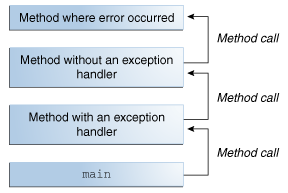
\includegraphics[width=0.8\linewidth]{figs/exceptions-callstack.png}

  	\column{.50\textwidth}
		Call stack: Sequence of invoked methods
	\end{columns}
\end{frame}

\begin{frame}{Exceptions}{Exception definition (III)}
    \begin{columns}
 	   \column{.60\textwidth}
		\centering Exception handling
		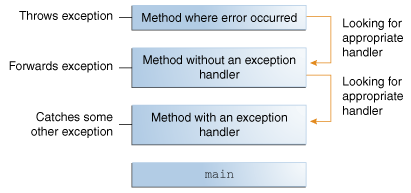
\includegraphics[width=0.8\linewidth]{figs/exceptions-errorOccurs.png}

  	\column{.60\textwidth}
		When an error happens ...
		\begin{enumerate}
		\item An exception is thrown
		\item Code execution is stopped
		\item The JVM goes back in the call stack
		\item When the JVM finds an exception handler, it is executed
		\end{enumerate}
		The exception handler catches the exception, the program finishes otherwise
	\end{columns}
\end{frame}

\begin{frame}{Exceptions}{Exception definition (IV)}
	\lstinputlisting{code/stack.txt}
\end{frame}

\subsection{try-catch}
\begin{frame}{Exceptions}{try-catch (I)}
	Handling an exception requires a try-catch statement
	\begin{itemize}
		\item try: Encloses the vulnerable code
		\item catch: Code that handles the exception
	\end{itemize}

    \begin{columns}
 	   \column{.60\textwidth}
	\begin{block}{try-catch statement}
	\vspace{-0.2cm}
		\lstinputlisting[language=java, basicstyle=\ttfamily\scriptsize]{code/try-catch.java}
	\vspace{-0.2cm}
	\end{block}
	\end{columns}
\end{frame}

\begin{frame}[plain]{Exceptions}{try-catch (II)}
	\vspace{-0.2cm}
    \begin{columns}
 	   \column{\textwidth}
	\begin{block}{ListOfNumbers.java (compilation error!)}
	\vspace{-0.2cm}
		\lstinputlisting[language=java, basicstyle=\ttfamily\scriptsize]{code/ListOfNumbers.java}
	\vspace{-0.2cm}
	\end{block}
	\end{columns}
\end{frame}

\begin{frame}[plain]{Exceptions}{try-catch (III)}
    \begin{columns}
 	   \column{\textwidth}
	\begin{block}{ListOfNumbers.java (corrected)}
	\vspace{-0.2cm}
		\lstinputlisting[language=java, basicstyle=\ttfamily\scriptsize]{code/ListOfNumbersGood.java}
	\vspace{-0.2cm}
	\end{block}
	\end{columns}
\end{frame}

\begin{frame}[plain]{Exceptions}{try-catch (IV)}
	\vspace{-0.2cm}
    \begin{columns}
 	   \column{\textwidth}
	\begin{block}{finally statement example}
	\vspace{-0.2cm}
		\lstinputlisting[language=java, basicstyle=\ttfamily\scriptsize]{code/finally.java}
	\vspace{-0.2cm}
	\end{block}
	\end{columns}
\end{frame}

\subsection{Exceptions thrown by a method}
\begin{frame}{Exceptions}{Exceptions thrown by a method (I)}
	Sometimes, we do not know how to handle an exception
		\begin{itemize}
		\item It is better to raise the exception
		\item Good practice: Handle exceptions when you know what to do
		\end{itemize}
	Methods can throw exceptions
		\begin{itemize}
		\item Forces handling errors
		\item Forces good programming
		\end{itemize}
	
	\begin{block}{Method throwing an exception}
	\vspace{-0.2cm}
		\lstinputlisting{code/method.java}
	\vspace{-0.2cm}
	\end{block}
\end{frame}

\begin{frame}{Exceptions}{Exceptions thrown by a method (II)}
	\begin{block}{Example}
	\vspace{-0.2cm}
		\lstinputlisting[language=java, basicstyle=\ttfamily\scriptsize]{code/throws.java}
	\vspace{-0.2cm}
	\end{block}
\end{frame}

\begin{frame}{Exceptions}{Exceptions thrown by a method (III)}
	Exception throwing
		\begin{itemize}
		\item Automatic: Certain operations like dividing by zero
		\item Manual: Using \alert{throw} statement
		\end{itemize}
	Remember: Exceptions are objects
	
	\begin{block}{Example}
	\vspace{-0.2cm}
		\lstinputlisting[language=java, basicstyle=\ttfamily\scriptsize]{code/throw.java}
	\vspace{-0.2cm}
	\end{block}
\end{frame}

\section{Basic I/O}
\subsection{Streams}
\begin{frame}{Basic I/O}{Streams (I)}
	All I/O operations in Java are based on \alert{streams}
		\begin{itemize}
			\item Stream: A sequence of data
			\item Input and output streams
		\end{itemize}

    \begin{columns}
 	   \column{.50\textwidth}
		\centering \textit{Input stream}
		\vspace{-0.2cm}
		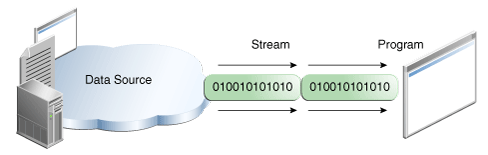
\includegraphics[width=\linewidth]{figs/io-ins.png}

  		\column{.50\textwidth}
		\centering \textit{Output stream}
		\vspace{-0.2cm}
		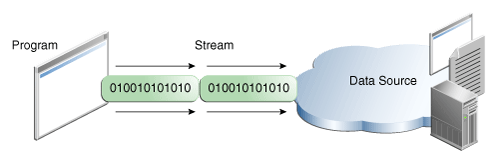
\includegraphics[width=\linewidth]{figs/io-outs.png}
	\end{columns}

    \bigskip
	Data may come from or go to anywhere
		\begin{itemize}
			\item File, device, network, ...
		\end{itemize}


\end{frame}

\begin{frame}[plain]{Basic I/O}{Streams (II)}
    \begin{columns}
 	   \column{.20\textwidth}
 	   \column{.50\textwidth}
		\vspace{-0.2cm}
		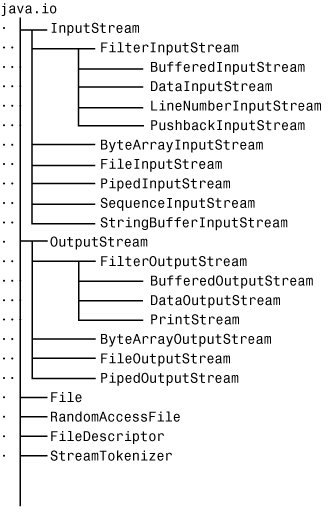
\includegraphics[width=0.9\linewidth]{figs/f13-1.png}\\
		\centering \tiny \href{http://www.webbasedprogramming.com/JAVA-Developers-Guide}{(Source)}

 	   \column{.40\textwidth}
	   	Java I/O has a complex class hierarchy
		\\
		\bigskip
	\end{columns}
\end{frame}

\subsection{User I/O}
\begin{frame}{Basic I/O}{User I/O (I)}
	By default, JVM has three streams:
		\begin{itemize}
		\item Input stream (\texttt{System.in}): Class \texttt{InputStream}
		\item Output stream (\texttt{System.out}): Class \texttt{PrintStream}
		\item Error stream (\texttt{System.err}): Class \texttt{PrintStream}
		\end{itemize}
	Problem: \texttt{InputStream} reads bytes, but not characters or strings
		\begin{itemize}
			\item The solution is to transform it into a \texttt{BufferedReader} object
		\end{itemize}
\end{frame}

\begin{frame}[shrink]{Basic I/O}{User I/O (II)}
	\vspace{-0.2cm}
	\begin{block}{IO Example}
	\vspace{-0.2cm}
		\lstinputlisting[language=java, basicstyle=\ttfamily\scriptsize]{code/io.java}
	\vspace{-0.2cm}
	\end{block}
\end{frame}

\section{Java Collections}
\subsection{Introduction}
\begin{frame}{Java Collections}{Introduction}
	Programming is about information representation
	\begin{itemize}
		\item Simple data are easy to represent:
		\begin{itemize}
			\item Numbers, characters, strings, etc
		\end{itemize}
	\end{itemize}
	Reality uses to be more complicated: Classes
	\begin{itemize}
		\item How can we store several objects?
		\item How can we represent complex data?
	\end{itemize}
	We need more powerful mechanisms to store information: Data structures
\end{frame}

\subsection{Data structures}
\begin{frame}[fragile]{Java Collections}{Data structures: Array}
    \begin{columns}
 	   \column{.50\textwidth}
		\begin{center}
		Vector (1-D array)

		\vspace{-0.2cm}

		\begin{tikzpicture} [nodes in empty cells, 
			nodes={minimum width=0.5cm, minimum height=0.5cm}, 
			row sep=-\pgflinewidth, column sep=-\pgflinewidth]
		border/.style={draw}
		\matrix(vector)[matrix of nodes, 
		row 1/.style={nodes={draw=none, minimum width=0.3cm}},
		nodes={draw}]
{
   	\tiny{0} & \tiny{1} & \tiny{2} & \tiny{3}\\
 	$a_{0}$ & $a_{1}$ & $a_{2}$ & $a_{3}$\\
};
		\end{tikzpicture}

		\bigskip

		Matrix
		\vspace{-0.2cm}

		\begin{tikzpicture} [nodes in empty cells, 
			nodes={minimum width=0.5cm, minimum height=0.5cm}, 
			row sep=-\pgflinewidth, column sep=-\pgflinewidth]
		border/.style={draw}
\matrix (matrix)[matrix of nodes, column 1/.style={nodes={draw=none, minimum width=0.3cm,  minimum height=0.3cm}}, 
		row 1/.style={nodes={draw=none, minimum width=0.3cm}},
		nodes={draw}]
{
   	& \tiny{0} & \tiny{1} & \tiny{2} & \tiny{3}\\
 \tiny{0} & $a_{0,0}$ & $a_{0,1}$ & $a_{0,2}$ & $a_{0,3}$\\
 \tiny{1} & $a_{1,0}$ & $a_{1,1}$ & $a_{1,2}$ & $a_{1,3}$\\
 \tiny{2} & $a_{2,0}$ & $a_{2,1}$ & $a_{2,2}$ & $a_{2,3}$\\
};

		\end{tikzpicture}
		\end{center}

  		\column{.50\textwidth}
		Advantajes:
		\begin{itemize}
			\item Very fast
			\item No extra memory
			\item Native language support
		\end{itemize}

		Disadvantajes:
		\begin{itemize}
			\item Fixed size
		\end{itemize}
	\end{columns}
\end{frame}

\begin{frame}[fragile]{Java Collections}{Data structures: Stack and queue}
    \begin{columns}
 	   \column{.50\textwidth}
		\begin{center}
		Stack\\
		\bigskip

		\begin{tikzpicture}[draw, minimum width=1cm, minimum height=0.5cm]
			%\draw[help lines] (-3,-2) grid (3,2);
			\node[draw] (in) at (-1,2) {};
			\node[draw] (out) at (1,2) {};
			\matrix (queue)[matrix of nodes, nodes={draw, nodes={draw}}, nodes in empty cells]
			{
  				\\ \\ \\ \\
			};

			\draw[-latex] (0.25,1) .. controls (0.25,1.5) and (1,1.5) .. (out.south);
			\draw[-latex] (in.south) .. controls (-1, 1.5) and (-0.25,1.5) .. (-0.25,1);
		\end{tikzpicture}
		\end{center}
		
		Operations
		\begin{itemize}
			\item \texttt{pop()} and \texttt{push()}
		\end{itemize}

  		\column{.50\textwidth}
		\begin{center}
		Queue\\
		\bigskip

		\begin{tikzpicture}[draw, minimum width=1cm, minimum height=0.5cm]
			%\draw[help lines] (-3,-2) grid (3,2);
			\node[draw] (in) at (-1,2) {};
			\node[draw] (out) at (1,-2) {};
			\matrix (queue)[matrix of nodes, nodes={draw, nodes={draw}}, nodes in empty cells]
			{
  				\\ \\ \\ \\
			};

			\draw[-latex] (0.25,-1) .. controls (0.25,-1.25) and (1,-1.25) .. (out.north);
			\draw[-latex] (in.south) .. controls (-1, 1.5) and (-0.25,1.5) .. (-0.25,1);
		\end{tikzpicture}
		\end{center}

		\vspace{-0.5cm}
		Operations
		\begin{itemize}
			\item \texttt{enqueue()} and \texttt{dequeue()}
		\end{itemize}
	\end{columns}
\end{frame}


\begin{frame}[fragile]{Java Collections}{Data structures: Lists}

    \begin{columns}
 	   \column{.50\textwidth}
	\begin{center}
	Linked list

	\newcommand{\chainlabel}[2]{\path [<-, draw, shorten >=10pt] (#1) |- node [at end] {#2} ++(-0.5,0.5);}
	\begin{tikzpicture}[every node/.style={rectangle split, rectangle split parts=2, rectangle split horizontal,minimum height=14pt}, node distance=1em, start chain,
	 every join/.style={->, shorten <=-4.5pt}]

	  \node[draw, on chain, join] {   };
	  \node[draw, on chain, join] {   };
	  \node[draw, on chain, join] {};
	  \chainlabel{chain-1.one north}{};
	\end{tikzpicture} 
	\end{center}
 	   \column{.50\textwidth}
		Operations
		\begin{itemize}
		\item \texttt{put()} and \texttt{get()}
		\item \texttt{remove()}
		\end{itemize}
		(List in Python)
	\end{columns}

    \begin{columns}
 	   \column{.50\textwidth}
	\begin{center}
	Hash table\\

	\begin{tikzpicture} [nodes={minimum width=0.8cm, minimum height=0.8cm}, 
		row sep=-\pgflinewidth, column sep=-\pgflinewidth]
	\matrix (hash)[matrix of nodes, nodes={draw, anchor=center}]
	{
	 Key1 & Value1 \\
	 Key2 & Value2 \\
	 Key3 & Value3 \\
	};
	\end{tikzpicture}

	\end{center}
 	   \column{.50\textwidth}
		Operations
		\begin{itemize}
		\item \texttt{put()} and \texttt{get()}
		\item \texttt{remove()}
		\end{itemize}
		(Dictionary in Python)
	\end{columns}
\end{frame}

\begin{frame}{Java Collections}{Data structures: Trees (I)}
	\begin{center}
		Trees
	\end{center}

	\vspace{-0.8cm}

    \begin{columns}
 	   \column{.50\textwidth}

	   	\begin{center}
		\begin{tikzpicture}[level distance=1.3cm,
		  level 1/.style={sibling distance=3cm, level distance=1cm},
		  level 2/.style={sibling distance=1.5cm, level distance=0.8cm}]
		  \node {Root}
		      child {node {Child}
		      child {node {Node}}
		      child {node {Node}}
		  }
		      child {node {Level 2}
		      child {node {Level 3}}
		      child {node {Level 3}}
		 };
		\end{tikzpicture}
		\end{center}

		Operations
		\begin{itemize}
			\item \texttt{insert()} and \texttt{remove()}
			\item \texttt{search()}
		\end{itemize}

  		\column{.50\textwidth}

		\begin{center}

		\begin{tikzpicture}[level distance=1.3cm,
		  level 1/.style={sibling distance=3cm},
		  level 2/.style={sibling distance=1.5cm, level distance=1cm},
		  level 3/.style={sibling distance=1cm, level distance=0.8cm}]
		  \node {+}
		      child {node {x}
		      	child {node {2}}
		      	child {node {+}
				  child {node {8}}
				  child {node {6}}
				}
		  	  }
		      child {node {5}
		 };
		\end{tikzpicture}
		\begin{equation*}
			2*(8+6)+5
		\end{equation*}
		\end{center}
	\end{columns}
\end{frame}

\begin{frame}{Java Collections}{Data structures: Trees (II)}
    \begin{columns}
 	   \column{.50\textwidth}
	   	\begin{center}
		\vspace{-0.2cm}
		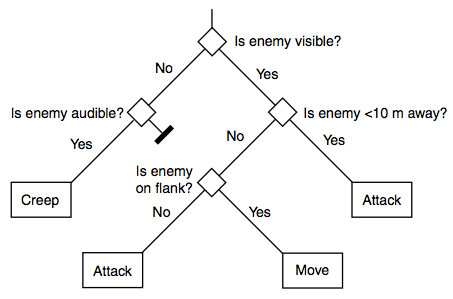
\includegraphics[width=0.9\linewidth]{figs/tree4.png}

		\bigskip

		\vspace{-0.2cm}
		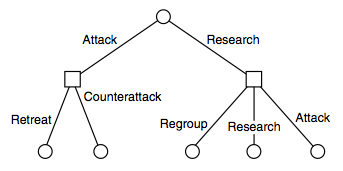
\includegraphics[width=0.9\linewidth]{figs/tree5.png}\\
		\tiny
		Source: Ian Millington, John Funge. ``\textit{Artificial Intelligence for Games}''. Ed. Morgan-Kaufmann. 2009.
		\end{center}

  		\column{.50\textwidth}
	   	\begin{center}
		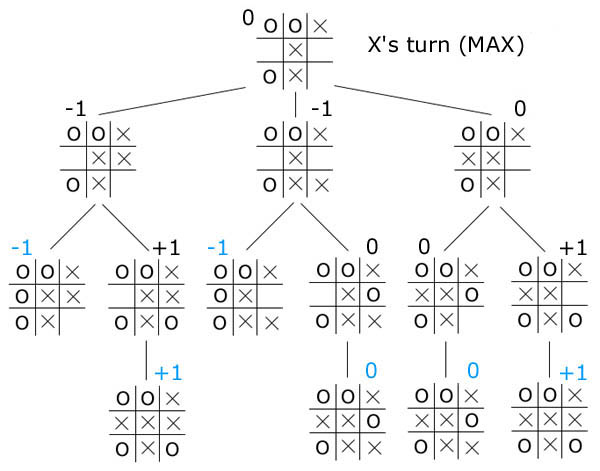
\includegraphics[width=\linewidth]{figs/raya.png}\\
		\tiny{\href{http://www.ocf.berkeley.edu/~yosenl/extras/alphabeta/alphabeta.html}{(Source)}}
	   	\end{center}
		\end{columns}
\end{frame}

\begin{frame}{Java Collections}{Data structures: Graphs}
	\begin{center}
	Graphs
	\end{center}

    \begin{columns}
 	   \column{.50\textwidth}
		\vspace{-0.2cm}
		\centering 

		\begin{tikzpicture}[scale=0.4]
    	\tikzstyle{node_style} = [circle,draw=black]
	    \tikzstyle{edge_style} = [draw=black]
		    \node[node_style] (v1) at (-2,2) {2};
		    \node[node_style] (v2) at (2,2) {3};
		    \node[node_style] (v3) at (4,0) {6};
		    \node[node_style] (v4) at (2,-2) {4};
		    \node[node_style] (v5) at (-2,-2) {5};
		    \node[node_style] (v6) at (-4,0) {1};
		    \draw[edge_style]  (v1) edge (v2);
		    \draw[edge_style]  (v2) edge (v3);
		    \draw[edge_style]  (v3) edge (v4);
		    \draw[edge_style]  (v4) edge (v5);
		    \draw[edge_style]  (v5) edge (v6);
		    \draw[edge_style]  (v6) edge (v1);
		    \draw[edge_style]  (v5) edge (v1);
		    \draw[edge_style]  (v5) edge (v2);
		    \draw[edge_style]  (v4) edge (v2);
	    \end{tikzpicture}
		\bigskip

		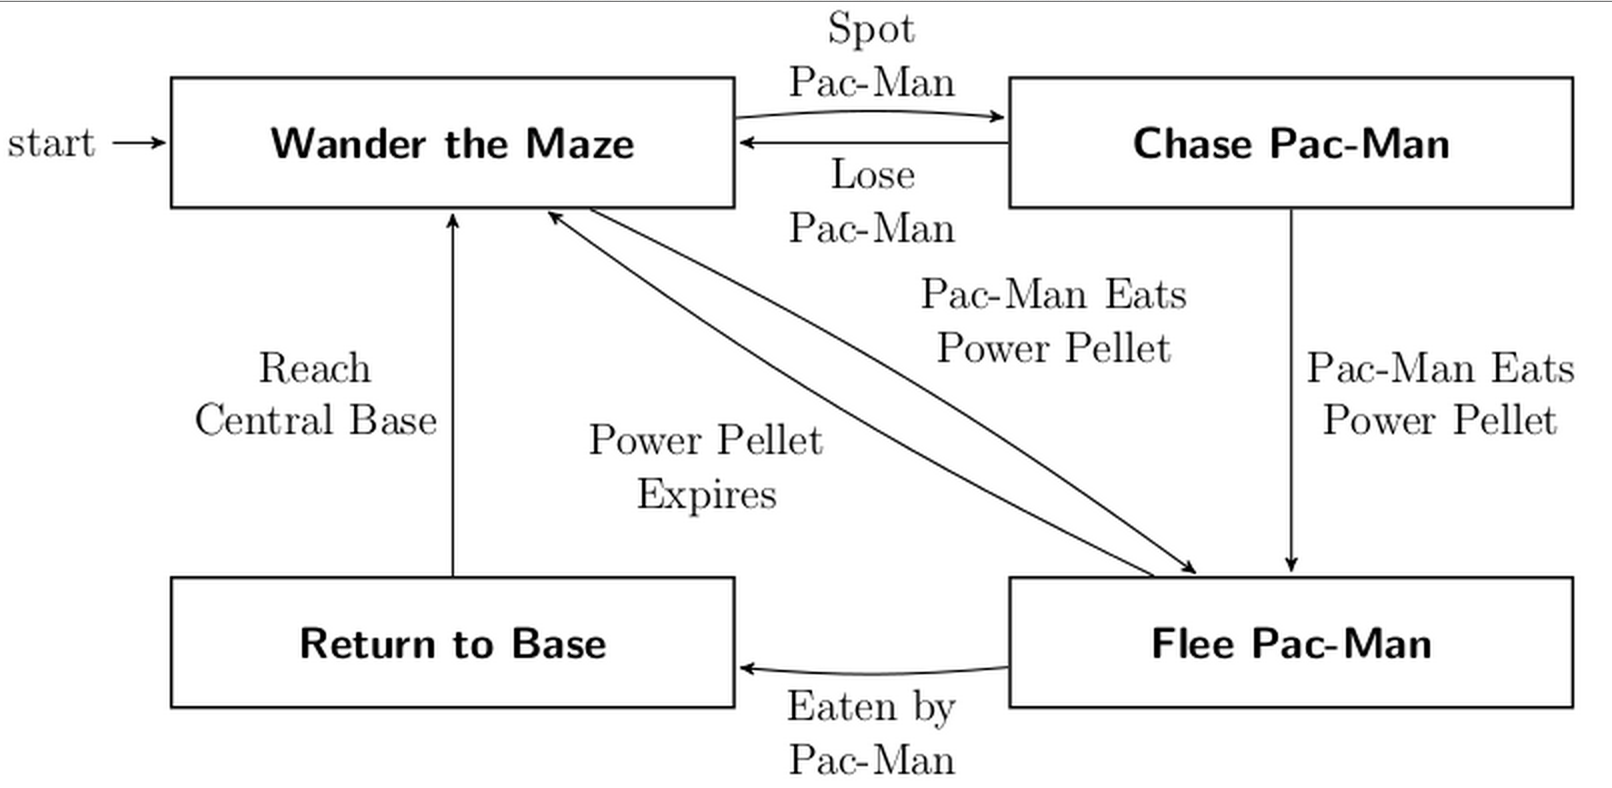
\includegraphics[width=\linewidth]{figs/fsm-pacman.png}\\
		\centering \tiny \href{http://bits.citrusbyte.com/state-design-pattern-with-ruby/}{(Source)}

  		\column{.50\textwidth}

		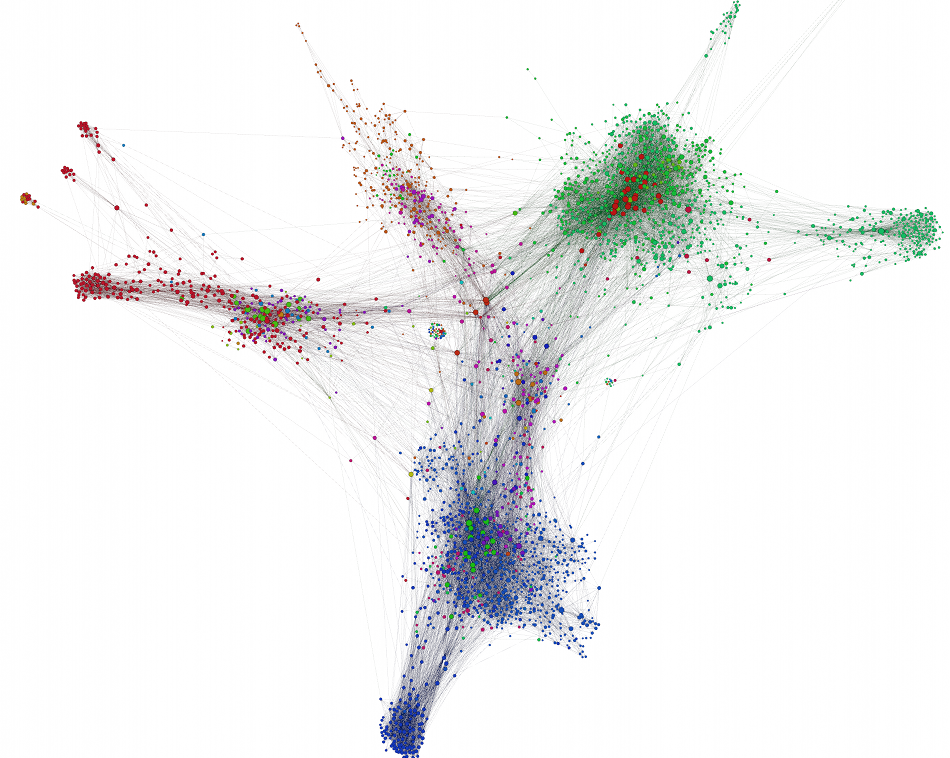
\includegraphics[width=\linewidth]{figs/layout2.png}\\
		\centering \tiny \href{https://gephi.org/features/}{(Source)}

		\end{columns}
\end{frame}


\subsection{Java Collections Framework}
\begin{frame}{Java Collections}{Java Collections Frakework}
	\begin{itemize}
		\item Java Collections is a framework that implements data structures
			\begin{itemize}
			\item It is \textit{very} useful
			\item Equivalent in Java to C++'s STL
			\end{itemize}
		\item A collection is a group of objects ... regardless of their class
		\item Three components
			\begin{enumerate}
			\item \textit{Interfaces}: Exposes the collection interface
			\item \textit{Implementations}: The implementation of a interface
			\item \textit{Algorithms}: Useful operations like sorting
			\end{enumerate}
	\end{itemize}
\end{frame}

\begin{frame}{Java Collections}{Java Collections Frakework: Interfaces}
	\begin{center}
	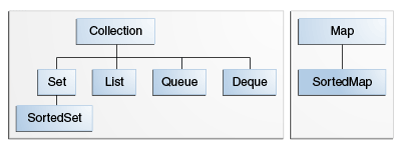
\includegraphics[width=0.6\linewidth]{figs/colls-coreInterfaces.png}\\
	\tiny \href{http://docs.oracle.com/javase/tutorial/collections/interfaces/index.html}{(Source)}
	\end{center}

	\begin{itemize}
		\item \textbf{Collection}: The root of the hierarchy
		\item \textbf{Set}: A collection without duplicates, not sorted
		\begin{itemize}
		\item \textbf{SortedSet}: A set with sorted elements
		\end{itemize}
		\item \textbf{List}: Ordered with duplicates and positions
		\item \textbf{Queue}: Insertion and extraction only
		\item \textbf{Map}: Key-value data structure, no duplicates, not sorted
		\begin{itemize}
		\item \textbf{SortedMap}: A map with order
		\end{itemize}
	\end{itemize}
\end{frame}

\begin{frame}{Java Collections}{Java Collections Frakework: Collection interface}
	Methods in the \texttt{Collection} interface
	\begin{itemize}
		\item \texttt{int size();}
		\item \texttt{boolean isEmpty();}
		\item \texttt{boolean contains(Object element);}
		\item \texttt{boolean add(E element);}
		\item \texttt{boolean remove(Object element);}
		\item \texttt{Object[] toArray();}
	\end{itemize}
	
	\begin{block}{Collection iteration}
	\vspace{-0.2cm}
		\lstinputlisting{code/Collection.java}
	\vspace{-0.2cm}
	\end{block}

\end{frame}

\begin{frame}{Java Collections}{Java Collections Frakework: Set interface}
	\begin{itemize}
	\item Same methods than \texttt{Collection}, no duplicates
	\item Implementations:
	\begin{itemize}
	\item \texttt{HashSet}, \texttt{TreeSet}, \texttt{LinkedHashSet}
	\end{itemize}
	\end{itemize}
	
	\vspace{-0.2cm}
	\begin{block}{FindDups}
	\vspace{-0.2cm}
		\lstinputlisting[language=java, basicstyle=\ttfamily\scriptsize]{code/Set.java}
	\vspace{-0.2cm}
	\end{block}

\end{frame}

\begin{frame}{Java Collections}{Java Collections Frakework: List interface}
	Same methods than \texttt{Collection}, no duplicates, ordered
	\begin{itemize}
		\item \texttt{E get(int index);}
		\item \texttt{E set(int index, E element);}
		\item \texttt{int indexOf(Object o);}
		\item \texttt{int lastIndexOf(Object o);}
	\end{itemize}
	Implementations: \texttt{ArrayList} and \texttt{LinkedList}
	\begin{block}{List example}
	\vspace{-0.2cm}
		\lstinputlisting[language=java, basicstyle=\ttfamily\scriptsize]{code/List.java}
	\vspace{-0.2cm}
	\end{block}
\end{frame}

\begin{frame}{Java Collections}{Java Collections Frakework: Map interface (I)}
	Stores key-value pairs, same methods than \texttt{Collection}, and new ones:
	\begin{itemize}
		\item \texttt{V put(K key, V value);}
		\item \texttt{V get(Object key);}
		\item \texttt{V remove(Object key);}
		\item \texttt{boolean containsKey(Object key);}
		\item \texttt{boolean containsValue(Object value);}
	\end{itemize}
	Implementations: \texttt{HashMap}, \texttt{TreeMap} and \texttt{LinkedHashMap}
\end{frame}

\begin{frame}{Java Collections}{Java Collections Frakework: Map interface (II)}
	\begin{block}{Freq.java}
	\vspace{-0.2cm}
		\lstinputlisting[language=java, basicstyle=\ttfamily\scriptsize]{code/Map.java}
	\vspace{-0.2cm}
	\end{block}
\end{frame}


\end{document}
